\documentclass[border=10pt]{standalone}
\usepackage{verbatim}
\usepackage{pgfplots}
\pgfplotsset{compat=1.14}

% stars_count = 512;
% max_time = 2.5
% steps = {0.1, 0.1 / 8, 0.1 / (8 * 8), 0.1 / (8 * 8 * 8), 0.1 / (8 * 8 * 8 * 8), 0.1 / (8 * 8 * 8 * 8 * 8)};

\begin{document}

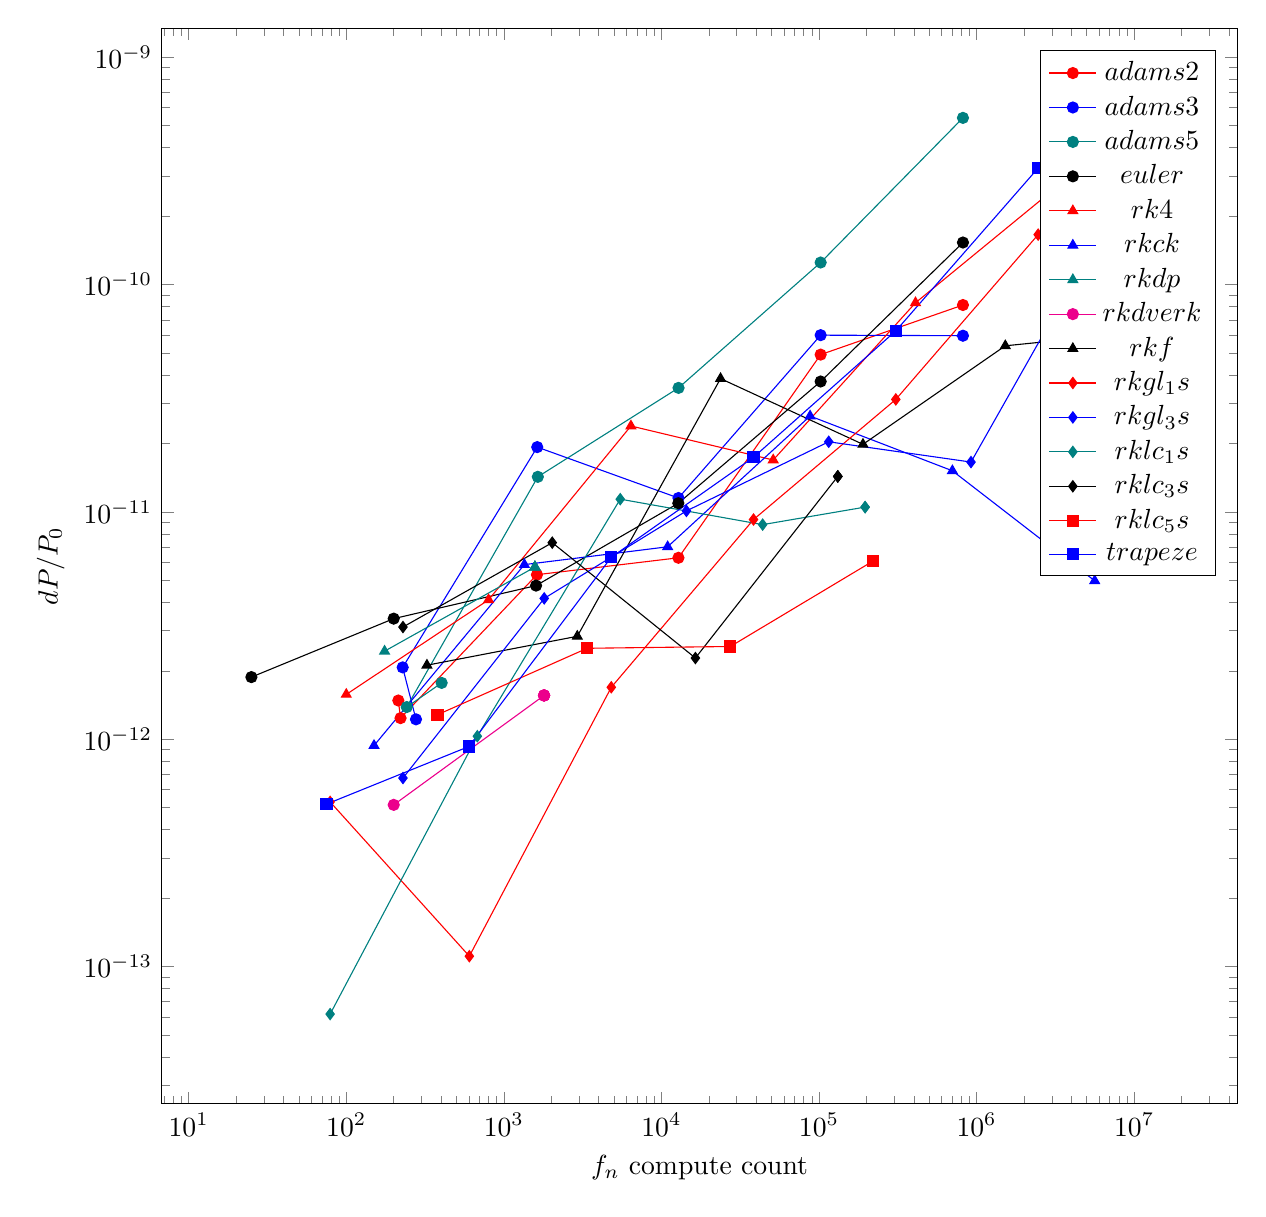
\begin{tikzpicture}
\begin{loglogaxis}[
    height=6in,
    width=6in,
    xlabel=$f_n$ compute count,
    ylabel=$dP/P_0$
]
\addplot [red,mark=*,solid] coordinates { (214, 1.48e-12) (221, 1.238e-12) (1622, 5.294e-12) (1.282e+04, 6.283e-12) (1.024e+05, 4.921e-11) (8.192e+05, 8.133e-11) };
\addplot [blue,mark=*,solid] coordinates { (277, 1.223e-12) (228, 2.07e-12) (1629, 1.928e-11) (1.283e+04, 1.151e-11) (1.024e+05, 5.993e-11) (8.192e+05, 5.959e-11) };
\addplot [teal,mark=*,solid] coordinates { (403, 1.769e-12) (242, 1.385e-12) (1643, 1.427e-11) (1.284e+04, 3.513e-11) (1.024e+05, 1.251e-10) (8.192e+05, 5.415e-10) };
\addplot [black,mark=*,solid] coordinates { (25, 1.876e-12) (200, 3.392e-12) (1601, 4.74e-12) (1.28e+04, 1.092e-11) (1.024e+05, 3.748e-11) (8.192e+05, 1.532e-10) };
\addplot [red,mark=triangle*,solid] coordinates { (100, 1.574e-12) (800, 4.104e-12) (6404, 2.388e-11) (5.12e+04, 1.692e-11) (4.096e+05, 8.318e-11) (3.277e+06, 2.714e-10) };
\addplot [blue,mark=triangle*,solid] coordinates { (150, 9.376e-13) (1350, 5.863e-12) (1.095e+04, 7.024e-12) (8.775e+04, 2.641e-11) (7.022e+05, 1.517e-11) (5.617e+06, 4.976e-12) };
\addplot [teal,mark=triangle*,solid] coordinates { (175, 2.439e-12) (1575, 5.72e-12) (1575, 5.72e-12) (1575, 5.72e-12) (1575, 5.72e-12) (1575, 5.72e-12) };
\addplot [magenta,mark=*,solid] coordinates { (200, 5.142e-13) (1800, 1.558e-12) (1800, 1.558e-12) (1800, 1.558e-12) (1800, 1.558e-12) (1800, 1.558e-12) };
\addplot [black,mark=triangle*,solid] coordinates { (325, 2.116e-12) (2925, 2.836e-12) (2.372e+04, 3.86e-11) (1.901e+05, 1.983e-11) (1.521e+06, 5.38e-11) (1.217e+07, 6.229e-11) };
\addplot [red,mark=diamond*,solid] coordinates { (79, 5.299e-13) (604, 1.11e-13) (4807, 1.692e-12) (3.841e+04, 9.255e-12) (3.072e+05, 3.126e-11) (2.458e+06, 1.66e-10) };
\addplot [blue,mark=diamond*,solid] coordinates { (229, 6.748e-13) (1804, 4.164e-12) (1.441e+04, 1.01e-11) (1.152e+05, 2.035e-11) (9.216e+05, 1.657e-11) (7.373e+06, 2.119e-10) };
\addplot [teal,mark=diamond*,solid] coordinates { (79, 6.174e-14) (679, 1.031e-12) (5479, 1.138e-11) (4.388e+04, 8.791e-12) (1.961e+05, 1.05e-11) (1.961e+05, 1.05e-11) };
\addplot [black,mark=diamond*,solid] coordinates { (229, 3.115e-12) (2029, 7.324e-12) (1.643e+04, 2.276e-12) (1.316e+05, 1.433e-11) (1.316e+05, 1.433e-11) (1.316e+05, 1.433e-11) };
\addplot [red,mark=square*,solid] coordinates { (379, 1.281e-12) (3379, 2.512e-12) (2.738e+04, 2.558e-12) (2.194e+05, 6.07e-12) (2.194e+05, 6.07e-12) (2.194e+05, 6.07e-12) };
\addplot [blue,mark=square*,solid] coordinates { (75, 5.183e-13) (600, 9.286e-13) (4803, 6.311e-12) (3.84e+04, 1.739e-11) (3.072e+05, 6.261e-11) (2.458e+06, 3.258e-10) };
\legend{$adams2$,$adams3$,$adams5$,$euler$,$rk4$,$rkck$,$rkdp$,$rkdverk$,$rkf$,$rkgl_1s$,$rkgl_3s$,$rklc_1s$,$rklc_3s$,$rklc_5s$,$trapeze$};
\end{loglogaxis}
\end{tikzpicture}

\end{document}
